\documentclass{article}
\usepackage[utf8]{inputenc}
\usepackage{url}
\usepackage{graphicx}
\usepackage[backend=biber,style=numeric]{biblatex}
\addbibresource{report.bib}
\begin{document}
   \begin{center}
       \vspace*{1cm}

       \textbf{Project Report}

       \vspace{0.5cm}
        Computer Based Tools and Applications (CMSC-6950)
   \end{center}
\begin{abstract}
Tidynamics is a simple python package which aids the computation of cross-correlation, autocorrelation and mean square displacement with less dependencies and in faster way. Here, I have demonstrated two computational task performed by using the functions tidynamics.correlate() and tidynamics.acf() from the package Tidynamics  using two datasets containing sensor data from smartphone accelerometer for six different activities. In addition, two visualization was performed using the output of the computational tasks to provide a better view of outcomes.
\end{abstract}

\section{Introduction to Tidynamics}

Tidynnamics is a package which provides an efficient implementation of Fast Correlation Algorithm (FCA) \cite{deBuy}. It provides functions to compute Autocorrelation, cross-correlation, mean square displacement and cross displacement. Routines in Tidynamics are bulilt using Numpy Arrays with a simple and user-friendly interface to ease its’ usage. For implementing FCA, Fast Fourier Transform (FFT) was required and for using FFT Numpy module numpy.fft() was used. 
The main advantage that the package Tidynamics provide is, it is very easy to install with ony one dependencies of Numpy. There are more packages to perform similar task that Tidynamics performs such as Numpy and Scipy. However, Tidynamics is more efficient in operation in comparison. For example, performing correlation require Numpy to loop over the regarding arrays directly which is not the case for Tidynamics. In terms of Scipy, it requires lots of dependencies if compared with Tidynamics. Moreover, numpy.correlate() and scipy.signal.correlate() differ from tidynamics.correlate() in terms of implementation too. 

\section{Performed Computational Task}
\textbf{Data Description}

Here I worked with two datasets named “Subject\_1\_data.csv” and “Subject\_2\_data.csv”. The datasets include data from smartphone accelerometer sensors while performing six activities. These two datasets both contain 5 columns and 348062 rows. The first column can be neglected. Columns \#2-\#4 contains data for Accelerometer X-axis, Accelerometer Y-axis, Accelerometer Z-axis respectively. The last column contains the name of the activities.


\vspace{1cm}
\textbf{First Task}

Here I computed correlation between column \#2 from subject\_1\_data.csv and subject\_2\_data.csv which are the data from X-axis of accelerometer sensor. At first I computed correlation between these two columns using three functions named tidynamics.correlate() from package tidynamics,  numpy.correlate() from package numpy and scipy.signal.correlate() from package scipy.
First the correlation was performed using the whole columns (348062 rows) and will record the time required to perform correlation for each function. Then the size of the columns was reduced by a factor of 10 (34806 rows) and the correlation was performed again as well as time was recorded. This process was repeated until the number of rows in the columns become less than 10 and greater than 1. After recording the time, a plot containing six subplots corresponding to six bar plots was created.   

\begin{figure}
\hspace*{-2cm}
    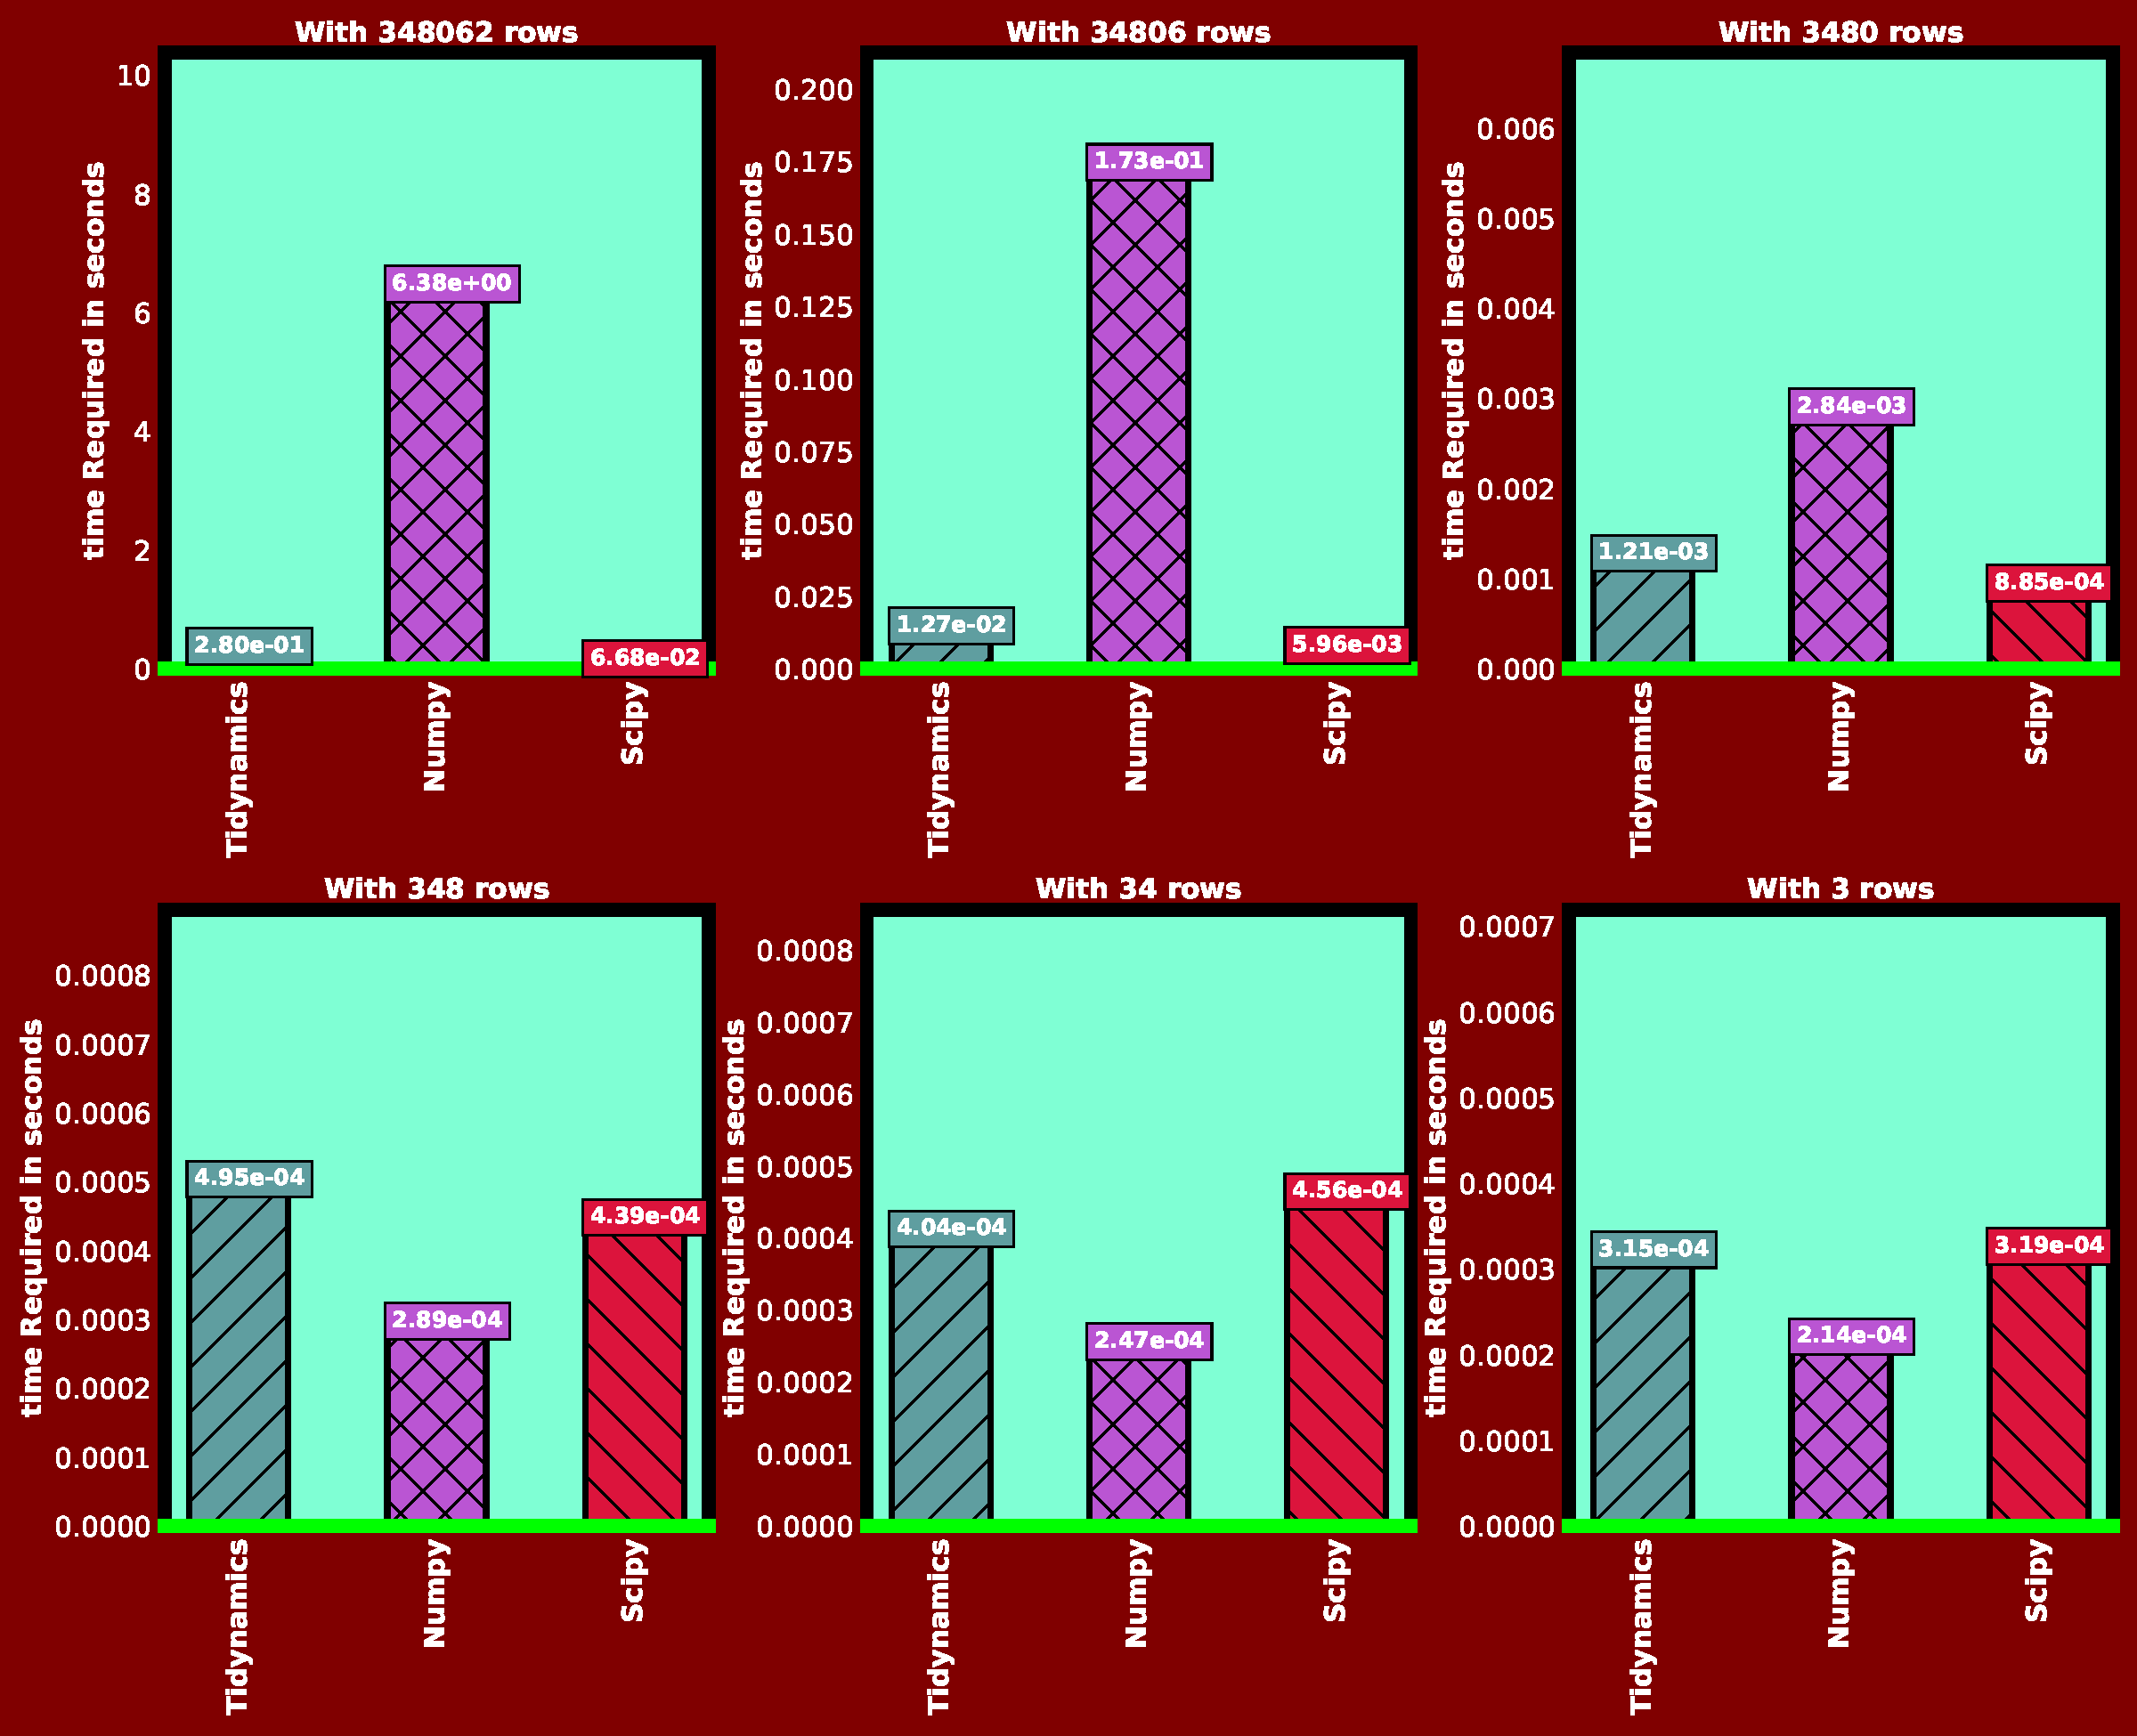
\includegraphics[width=16cm,height=10cm]{TimeComparison}
    \caption{Time Comparison for correlation among tidynamics, numpy and scipy}
    \label{fig:mesh1}
\end{figure}

figure \ref{fig:mesh1} contains the mentioned plot. Here each bar plot shows comparison between the time required by each function for different data size.

\vspace{0.5cm}
\textbf{Second Task}

In this task, we used the tidynamics.acf() function to compute autocorrelation of some data from the “Subject\_2\_data.csv” file. Autocorrelation means the correlation of some data with itself at different lags. For more information about autocorrelation, check this link https://nwfsc-timeseries.github.io/atsa-labs/sec-tslab-correlation-within-and-among-time-series.html 

Recall that the “Subject\_2\_data.csv” contains data for a tri-axial accelerometer for six different activities. For this task, I used 500 rows for each type of activity for columns \#2-\#4, which indicates the three axes of the accelerometer. As there are six different activities so there were six (500 by 3) dataframe I worked on. 

\begin{figure}
\hspace*{-2cm}
    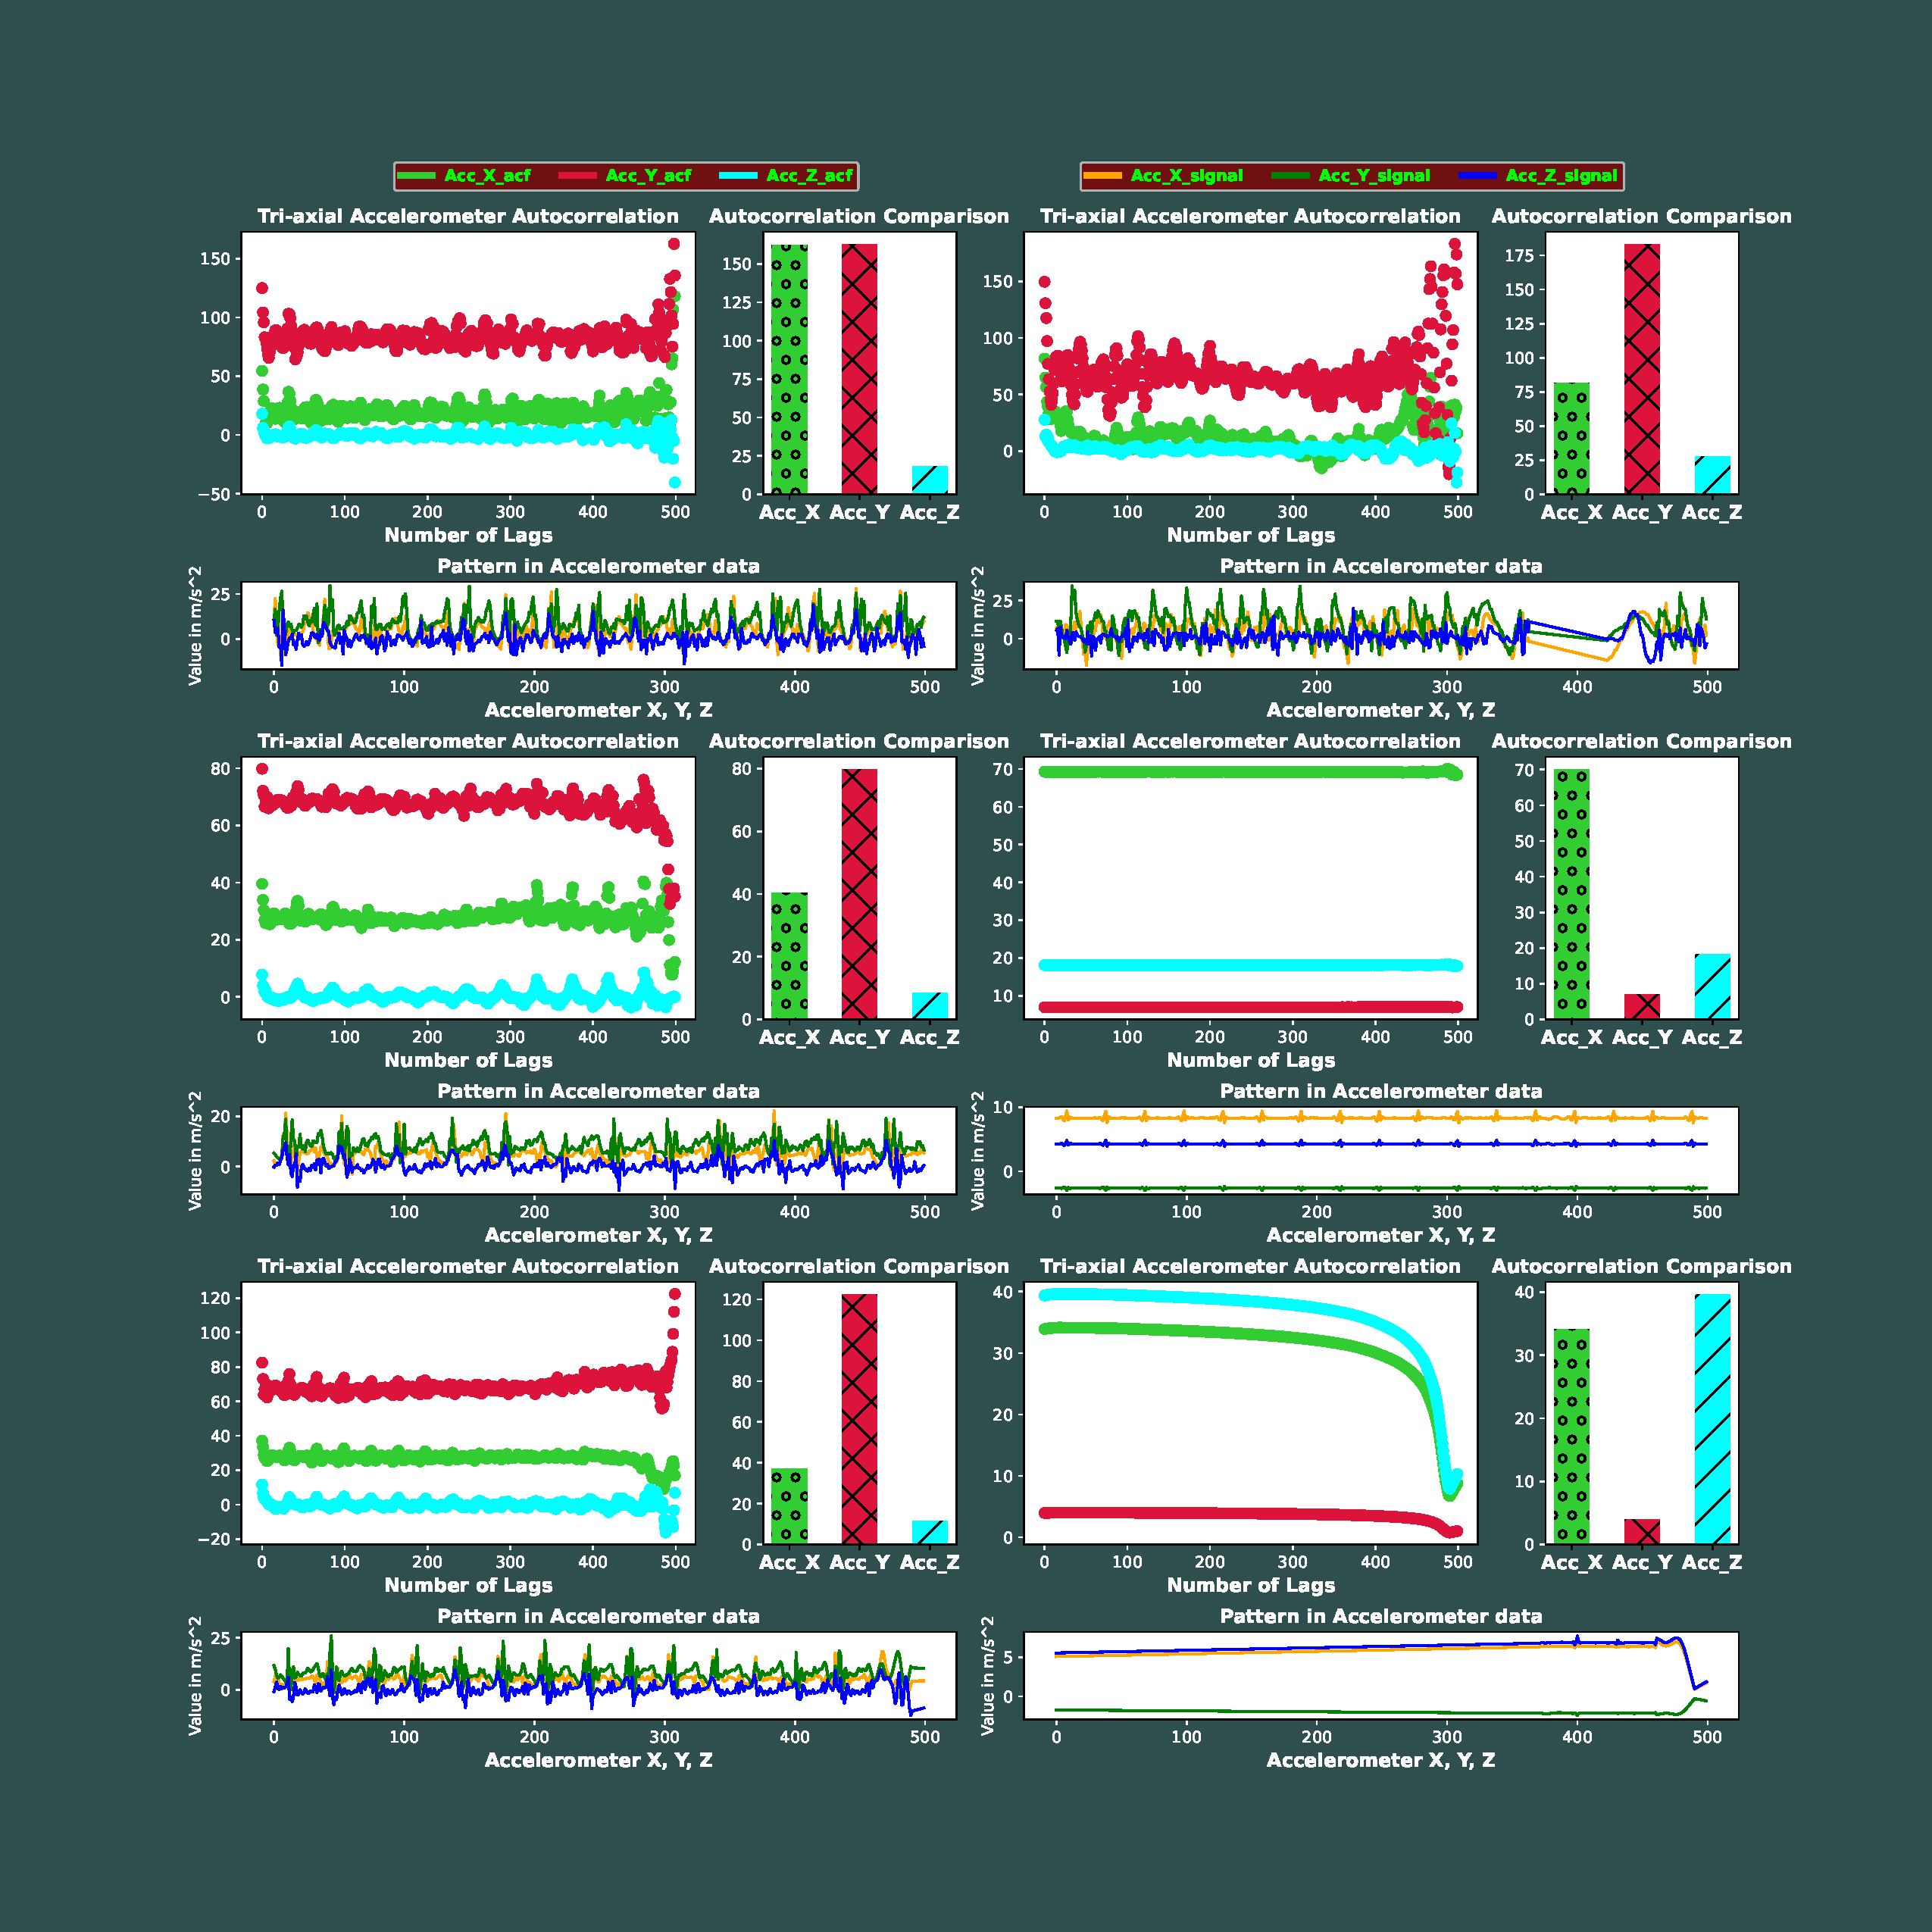
\includegraphics[width=16cm,height=17cm]{Acf_activities}
    \caption{Autocorrelation with Scatterplot, Autocorrelation comparison with vertical bar plot and raw signals with horizontal line plot}
    \label{fig:mesh2}
\end{figure}

Figure \ref{fig:mesh2} shows the outcome after performing task. There are total of 6 main subplots and each main subplot contains 3 subplots in Figure \ref{fig:mesh2}. So, we can see 18 plots in total (3 subplots for one activity type).
As described, there are 3 subplots for each type of activities where one plot is a scatter plot and it visualizes the autocorrelation of each axis of the tri-axial accelerometer with itself (correlation of x-axis with itself, correlation of y-axis with itself, correlation of y-axis with itself) for different time lags (lag 1 to lag 500). Another plot is there under the plot I just described as a horizontal rectangular plot. This shows the line plot of the raw values of all three accelerometer axes. Finally, the other plot is a bar plot, and it shows the maximum autocorrelation found for each axis.

\vspace{1cm}
\printbibliography
\end{document}

